\documentclass{article}
\usepackage[paperwidth=4in,paperheight=3in,margin=0.1in]{geometry}
\usepackage{tikz}

\begin{document}
\begin{center}
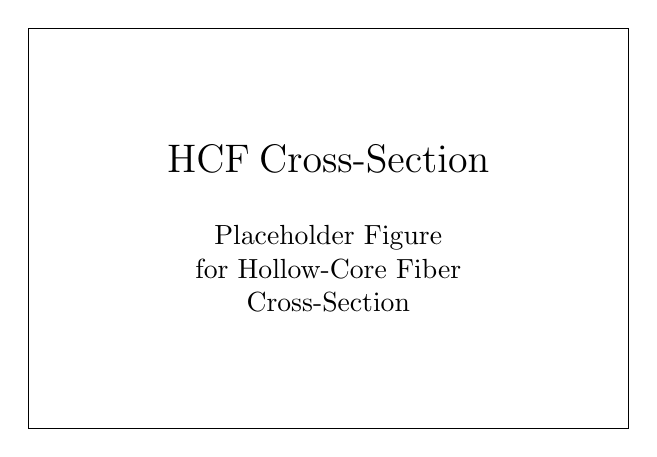
\begin{tikzpicture}
  \node[draw, rectangle, minimum width=3in, minimum height=2in, text width=2.5in, align=center] {
    \Large HCF Cross-Section\\[0.5cm]
    \normalsize Placeholder Figure\\
    for Hollow-Core Fiber\\
    Cross-Section
  };
\end{tikzpicture}
\end{center}
\end{document}
